\section{Basic Results of Complexity Theory}


\subsection{Linear Compression and Speedup}

\key{Big-Oh Notation} $g(n) \in O(f(n)) \Leftrightarrow \exists c > 0, \forall n,
g(n) \le cf(n)$.

\key{Theorem 5.1 (Space Compression with Tape Reduction).} For every k-tape
$S(n)$
space-bounded off-line Turing machine $M$ and constant $c > 0$, there exists a one-
tape $cS(n)$ space-bounded off-line Turing machine $N$ such that $L(M) = L(N)$.
Furthermore, if $M$ is deterministic, then so is $N$.

\key{Corollary 5.1.} The following identities hold:
\begin{align*}
\text{DSPACE}(S(n)) &= \text{DSPACE}(O(S(n)))\\
\text{NSPACE}(S(n)) &= \text{NSPACE}(O(S(n)))
\end{align*}
This implies DLBA = DSPACE($n$), and LBA = NSPACE($n$).

\key{Theorem 5.2 (Linear Speedup).} If $L$ is accepted by a k-tape $T(n)$ time-
bounded Turing machine $M$, $k > 1$, and if $n \in o(T(n))$, then for any $c
> 0$, $L$ is
accepted by a k-tape $cT(n)$ time-bounded Turing machine $N$. Furthermore, if
$M$ is
deterministic, then so is $N$.

\subsection{Constructible Functions}

\key{Space-constructible} There is an $S(n)$ space-bounded Turing
machine $M$ such that for each $n$ there is some input of length $n$ on which
$M$ uses
exactly $S(n)$ cells.

\key{Property of Space-constructible}

\begin{itemize}
  \item Space-constructible implies fully
    space-constructible for
    space bounds $S(n)$ such that $S(n) \ge n$.
  \item If $S_1(n)$ and $S_2(n)$ are space-constructible, then so are
    $S_1(n)S_2(n)$, $2^{S_1(n)}$ , and $S_1(n)^{S_2(n)}$
\end{itemize}

\subsection{Tape Reduction}

\key{Theorem 5.5} Let $M$ be a k-tape $T(n)$ time-bounded Turing machine
such that $n \in o(T(n))$. There is a one-tape $T^2(n)$ time-bounded
Turing machine
$N$ such that $L(N) = L(M)$. Furthermore, if $M$ is deterministic, then so is
$N$.

\key{Oblivious TM}A Turing machine is oblivious if the sequence of head moves on
the
Turing machine's tapes is the same for all input words of the same
length. That is,
for $t \ge 1$, the position of each of the heads after $t$ moves on an
input word $x$ depends on $t$ and $|x|$, but not on $x$.

\key{Theorem 5.6.} If $L$ is accepted by a k-tape $T(n)$ time-bounded
Turing machine $M$, then $L$ is accepted by an oblivious two-tape Turing machine
$N$ in time $O(T(n)logT(n))$. Furthermore, if $M$ is deterministic, then so is
$N$.

\key{Theorem 5.7.} If $L$ is accepted by a k-tape $T(n)$ time-bounded non-
deterministic Turing machine M, then there are a constant $c > 0$ and a two-tape
nondeterministic Turing machine $N$ that accepts $L$ such that for each word
$x \in L$,
the number of steps in the shortest computation of N on $x$ is at most $cT(n)$.

\subsection{Inclusion Relationships}

\key{Theorem 5.8.} For every function $f$ ,
DTIME($f$) $\subseteq$ DSPACE($f$) and NTIME($f$) $\subseteq$ NSPACE($f$)

\key{Theorem 5.9.} If $L$ is accepted by an $S(n)$ space-bounded Turing machine, 
$S(n) \ge log n$, then $L$ is accepted by an $S(n)$ space-bounded
Turing machine that halts on every input.

\key{Corollary 5.6.} For $S(n) \ge log(n)$,
DSPACE($S(n)$) $\subseteq$ $\bigcup \{$DTIME($c^{S(n)}) | c \ge 1 \}$

\key{Theorem 5.10.}  NTIME($T(n)$) $\in$ DSPACE($T(n)$).

\key{Corollary 5.7.} NP $\subseteq$ PSPACE.

\key{Theorem 5.11.} NTIME($T(n)$) $\subseteq$ $\bigcup$\{DTIME($c^{T(n)}| c \ge 1$\}.

\key{Corollary 5.8.} If $S$ is fully time-constructible and $S(n) \ge
log(n)$, then NSPACE($S(n)$) $\subseteq$ $\bigcup$ \{DTIME($c^{S(n)}|c \ge 1$\}).

\key{Theorem 5.13 (Savitch).} If $S$ is fully space-constructible and $S(n) \ge
log(n)$, then NSPACE($S(n)$) $\subseteq$ DSPACE($S^2(n)$).

\key{Corollary 5.9.}
\begin{align*}
  \text{PSPACE} &= \bigcup \{\text{DSPACE}(n^c) | c \ge 1\}\\
  &= \bigcup \{\text{NSPACE}(n^c) | c \ge 1\} \\
  \text{POLYLOGSPACE} &= \bigcup\{\text{DSPACE}(log(n)^c) | c \ge 1\}\\
  &= \bigcup \{\text{NSPACE}(log(n)^c) | c \ge 1\}
\end{align*}

\key{Corollary 5.10.}
\begin{align*}
\text{NSPACE}(n) &\subseteq \text{DSPACE}(n^2)\\
\text{NL} &\subseteq  \text{POLYLOGSPACE}.
\end{align*}

\subsubsection{Relations Between the Standard Classes}
\begin{figure}[H]
  \centering
  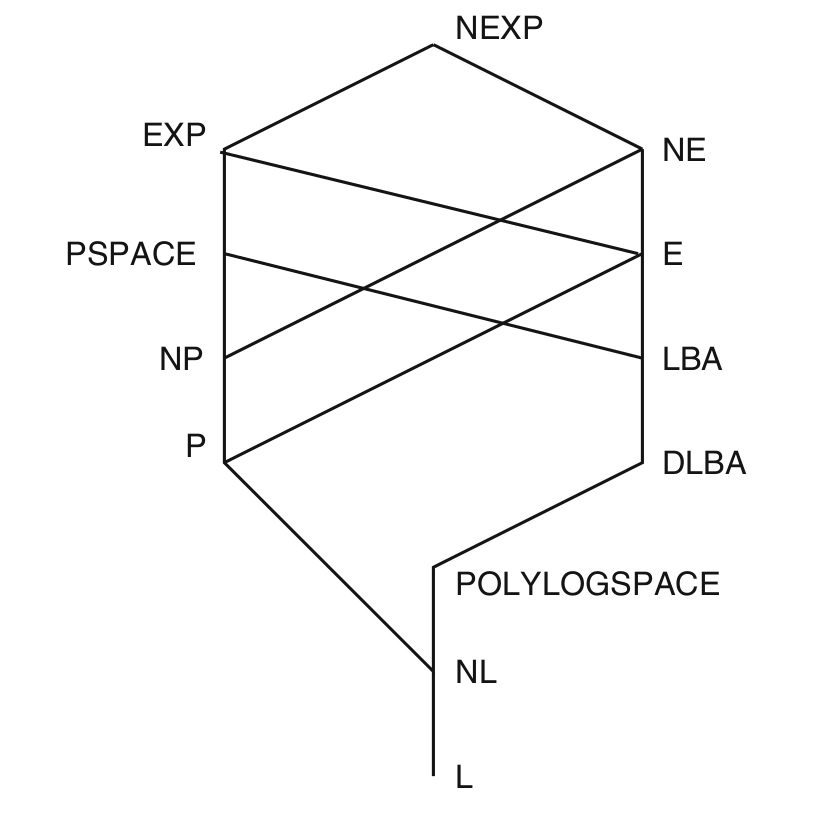
\includegraphics[width=0.38\textwidth]{hierarchy}
  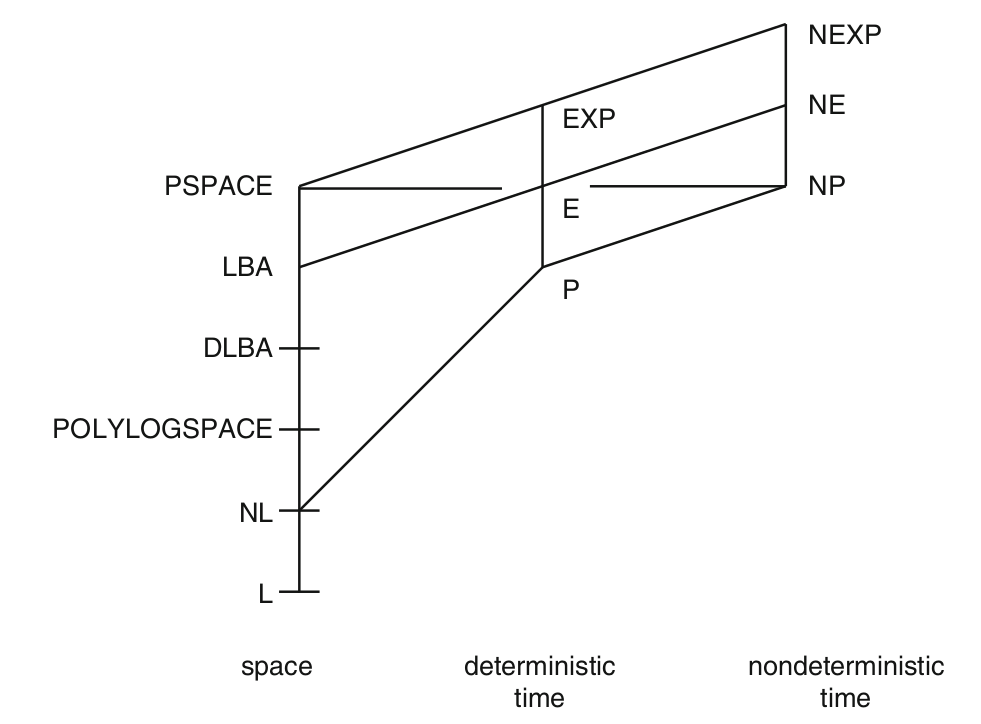
\includegraphics[width=0.6\textwidth]{hierarchy2}
\end{figure}

\key{Savitch (NSPACE($S(n)$) $\subseteq$ DSPACE($S^2(n)$))}
\begin{itemize}
  \item NL $\subseteq$ POLYLOGSPACE
  \item LBA $\subseteq$ PSPACE
\end{itemize}

\key{Space Hierarchy}
\begin{itemize}
  \item POLYLOGSPACE $\subseteq$ DLBA
\end{itemize}

\key{DSPACE($S(n)$) $\subseteq$ $\bigcup\{$DTIME($c^{S(n)})|c \ge 1\}$}
\begin{itemize}
  \item L $\subseteq$ P
  \item DLBA $\subseteq$ E
  \item PSPACE $\subseteq$ EXP
\end{itemize}

\key{NSPACE($S(n)$) $\subseteq$ $\bigcup\{$DTIME($c^{S(n)})|c \ge 1\}$.}
\begin{itemize}
  \item NL $\subseteq$ P 
  \item LBA $\subseteq$ E
\end{itemize}

\key{NTIME($S(n)$) $\subseteq$ DSPACE($S(n)$)}
\begin{itemize}
  \item NP $\subseteq$ PSPACE
\end{itemize}


\subsection{Separation Results}

\key{Theorem 5.15 (Space Hierarchy Theorem ).} Let $S(n)$ be fully space-
constructible. There is a language $L \in \text{DSPACE}(S(n))$ such that for every function
$S'(n)$, if $S'(n) \in o(S(n))$, then $L \notin \text{DSPACE}(S(n))$.

\key{Corollary 5.13.} $L \subset$ POLYLOGSPACE, POLYLOGSPACE $\subset$ DLBA, and DLBA
$\subset$ PSPACE.
\begin{align*}
\text{POLYLOGSPACE} &= \bigcup \{\text{DSPACE}((logn)^k ) | k \ge 1\}\\
&\subseteq \text{DSPACE}(n^\frac{1}{2})\\
&\subset \text{DLBA}.
\end{align*}

\key{Corollary 5.14.} LBA $\subset$ PSPACE.
\begin{align*}
\text{LBA} &= \text{NSPACE}(n), \text{by Corollary 5.1} \\
& \subseteq \text{DSPACE}(n^2 ), \text{by Theorem 5.13} \\
& \subset \text{DSPACE}(n^3 ), \text{by Theorem 5.15} \\
& \subseteq \text{PSPACE}.
\end{align*}

\key{Theorem 5.16 (Time Hierarchy Theorem).} Let $T$ be a fully time-constructible
function and assume that there exists a function $T'(n)$ so that
$T'(n)log(T'(n)) \in o(T(n))$.
Then there is a language $L \in \text{DTIME}(T(n))$ such that for every function 
$T'(n)$ such that $T'(n)log(T'(n)) \in o(T(n))$, $L \notin \text{DTIME}(T'(n))$.

\key{Corollary 5.15.} For every constant $c > 0$, DTIME($n^c$) $\subset$ DTIME($n^{c+1}$) and
DTIME($2^{cn}$) $\subset$ DTIME($2^{(c+1)n}$).

\key{Corollary 5.16.} P $\subset$ E and E $\subset$ EXP.

\subsection{Translation Techniques and Padding}

\key{Lemma 5.2.} Let $S(n)$ and $f(n)$ be fully space-constructible functions, where
$S(n) \ge n$ and $f(n) \ge n$. For a language $L$, define
$p(L) = \{x10^i | x \in L \text{ and }|x10^i | = f(|x|)\}$.
Then $L \in \text{NSPACE}(S(f(n))) \Leftrightarrow p(L) \in \text{NSPACE}(S(n))$.

\key{Theorem 5.17.} Let $S_1(n), S_2(n)$, and $f(n)$ be fully space-constructible functions,
where $S_1 (n) \ge n, S_2(n) \ge n$ and $f(n) \ge n$. Then
NSPACE($S_1(n)) \subseteq$ NSPACE($S_2(n)$) implies NSPACE($S_1(f(n)))
\subseteq$ NSPACE($S_2(f(n)))$.

\key{Example 5.5.} NSPACE($n^2$) $\subset$ NSPACE($n^3$).\\
Suppose for contradiction that NSPACE($n^3$) $\subseteq$ NSPACE($n^2$), then we 
have
\begin{align*}
  \text{NSPACE}(n^6) &\subseteq \text{NSPACE}(n^4) \text{ with } f(n)=n^2\\
  \text{NSPACE}(n^9) &\subseteq \text{NSPACE}(n^6) \text{ with } f(n)=n^3
\end{align*}
Then we have the following.
\begin{align*}
\text{NSPACE}(n^9) &\subseteq \text{NSPACE}(n^6) \\
&\subseteq \text{NSPACE}(n^4) \\
&\subseteq \text{DSPACE}(n^8), \text{ by Savitch theorem} \\
&\subset \text{DSPACE}(n^9), \text{by space hierarchy theorem} \\
&\subseteq \text{NSPACE}(n^9)
\end{align*}

\key{Example 5.6.} We use the analog of Theorem 5.17 for deterministic time to show
that DTIME($2^n$) $\subset$ DTIME($n2^n$).\\
Suppose for contradiction that DTIME($n2^n$) $\subseteq$ DTIME($2^n$), then we have 
\begin{align*}
\text{DTIME}(2^n2^{2^n}) &\subseteq \text{DTIME}(2^{2^n}) \text{ with } f(n) = 2^n\\
\text{DTIME}((n+2^n)2^{n+2^n}) &\subseteq \text{DTIME}(2^{n+2^n}) \text{ with }
f(n) = n+2^n\\
\text{DTIME}((n+2^n)2^{n}2^{2^n}) &\subseteq \text{DTIME}(2^{2^n}) \text{
combine above two.}
\end{align*}
Which violate the time hierarchy theorem.

\subsubsection{Tally Languages}

\key{Definition} For $L \in \Sigma^*$, let Tally(L) = $\{1^{n(w)} | w \in L\}$.

\key{Theorem 5.18.} NE $\subseteq$ E if and only if every tally language in NP belongs
to P.

\key{Corollary 5.17.} P = NP implies E = NE.
